\let\negmedspace\undefined
\let\negthickspace\undefined
\documentclass[journal]{IEEEtran}
\usepackage[a4paper, margin=10mm, onecolumn]{geometry}
\usepackage{lmodern} % Ensure lmodern is loaded for pdflatex
\usepackage{tfrupee} % Include tfrupee package

\setlength{\headheight}{1cm} % Set the height of the header box
\setlength{\headsep}{0mm}  % Set the distance between the header box and the top of the text

\usepackage{gvv-book}
\usepackage{gvv}
\usepackage{cite}
\usepackage{amsmath,amssymb,amsfonts,amsthm}
\usepackage{algorithmic}
\usepackage{graphicx}
\usepackage{float}
\usepackage{textcomp}
\usepackage{xcolor}
\usepackage{txfonts}
\usepackage{listings}
\usepackage{enumitem}
\usepackage{mathtools}
\usepackage{gensymb}
\usepackage{comment}
\usepackage[breaklinks=true]{hyperref}
\usepackage{tkz-euclide} 
\usepackage{listings}
% \usepackage{gvv}                                        
\def\inputGnumericTable{}                                 
\usepackage[latin1]{inputenc}                                
\usepackage{color}                                            
\usepackage{array}                                            
\usepackage{longtable}                                       
\usepackage{calc}                                             
\usepackage{multirow}                                         
\usepackage{hhline}                                           
\usepackage{ifthen}                                           
\usepackage{lscape}
\usepackage{tikz}
\usetikzlibrary{patterns}

\begin{document}

\bibliographystyle{IEEEtran}
\vspace{3cm}

\title{4.7.61}
\author{EE25BTECH11064 - Yojit Manral}

\maketitle
% \maketitle
% \newpage
% \bigskip
{\let\newpage\relax\maketitle}
\renewcommand{\thefigure}{\theenumi}
\renewcommand{\thetable}{\theenumi}
\setlength{\intextsep}{10pt} % Space between text and float

\textbf{Question:}\\
Find the coordinates of the foot of the perpendicular drawn from the origin to the plane $2x - 3y + 4z - 6 = 0$

\textbf{Solution:}\\
$\rightarrow$ From the equation of a general plane,
\begin{align} \vec{n}^{T}\vec{x} = c \end{align}
$\rightarrow$ A vector perpendicular to the plane and passing through the origin can be given as \begin{align} \vec{y} = \alpha \vec{n} \end{align}
$\rightarrow$ The foot of perpendicular must be the intersection of (1) and (2)...
\begin{align}
    \vec{n}^{T} (\alpha \vec{n}) &= c \\
    \alpha \vec{n}^{T} \vec{n} &= c \\
    \alpha &= \frac{c}{\norm{\vec{n}}^{2}}
\end{align}
$\rightarrow$ Now we can find the foot of perpedicular as
\begin{align} \vec{x_\perp} = \alpha \vec{n} = \frac{c}{\norm{\vec{n}}^{2}} \vec{n} \end{align}
$\rightarrow$ Given that
\begin{align}
    \vec{n} = \myvec{2\\-3\\4} \implies \norm{\vec{n}}^{2} = 29 &&\text{and}&& c = 6 \\
    &\implies \vec{x_\perp} = \frac{6}{29} \myvec{2\\-3\\4} = \myvec{12/29\\-18/29\\24/29}
\end{align}
\begin{figure}[h!]
   \centering
   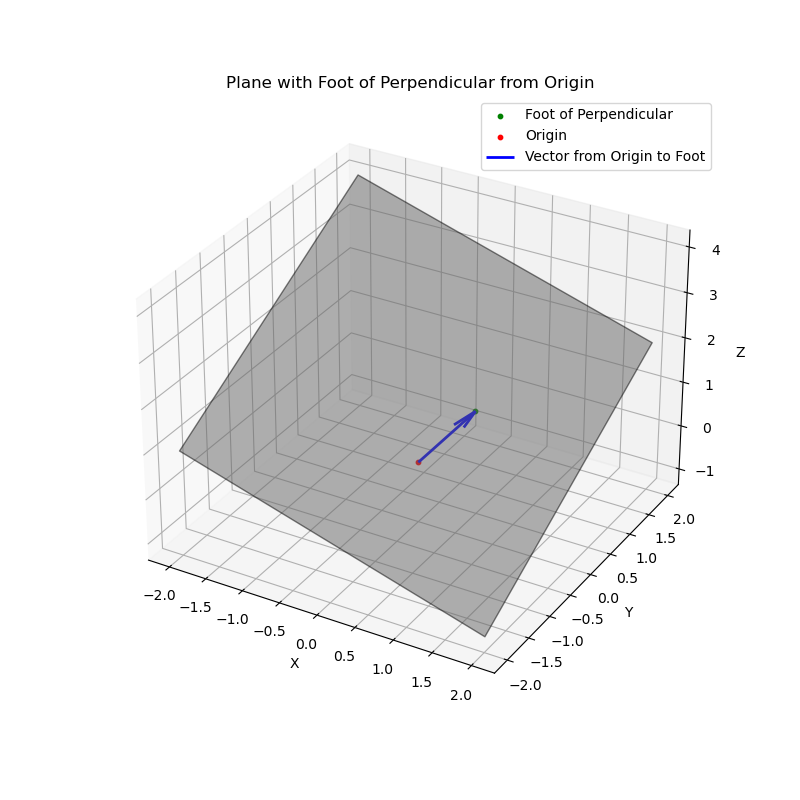
\includegraphics[width=0.6\linewidth]{figs/01.png}
   \caption{Foot of perpendicular of plane from origin}
   \label{Plot_1}
\end{figure}
\end{document}
